\documentclass[12pt]{article}
\usepackage[margin=2.5cm]{geometry}
\usepackage{enumerate}
\usepackage{amsfonts}
\usepackage{amsmath}
\usepackage{fancyhdr}
\usepackage{amsmath}
\usepackage{amssymb}
\usepackage{amsthm}
\usepackage{mdframed}
\usepackage{graphicx}
\usepackage{subcaption}
\usepackage{adjustbox}
\usepackage{listings}
\usepackage{xcolor}
\usepackage{booktabs}
\usepackage[utf]{kotex}
\usepackage{hyperref}

\definecolor{codegreen}{rgb}{0,0.6,0}
\definecolor{codegray}{rgb}{0.5,0.5,0.5}
\definecolor{codepurple}{rgb}{0.58,0,0.82}
\definecolor{backcolour}{rgb}{0.95,0.95,0.92}

\lstdefinestyle{mystyle}{
    backgroundcolor=\color{backcolour},
    commentstyle=\color{codegreen},
    keywordstyle=\color{magenta},
    numberstyle=\tiny\color{codegray},
    stringstyle=\color{codepurple},
    basicstyle=\ttfamily\footnotesize,
    breakatwhitespace=false,
    breaklines=true,
    captionpos=b,
    keepspaces=true,
    numbers=left,
    numbersep=5pt,
    showspaces=false,
    showstringspaces=false,
    showtabs=false,
    tabsize=1
}

\lstset{style=mystyle}

\pagestyle{fancy}
\renewcommand{\headrulewidth}{0.4pt}
\lhead{Team Treehouse}
\rhead{Querying Relational Databases Part 3 Notes}

\begin{document}
\title{Querying Relational Databases Part 3 Notes}
\author{Team Treehouse}
\maketitle

\bigskip

\section{One to Many Relationships}

\bigskip

\begin{itemize}
    \item Is most common type of relationship
    \item Is case where there is one table with many foreignkeys and not the other
    \item Foreign Key is always the many side

    \begin{center}
    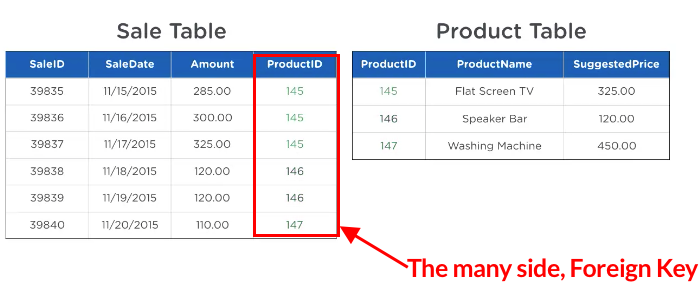
\includegraphics[width=0.8\linewidth]{images/part_3_notes_1.png}
    \end{center}
\end{itemize}

\bigskip

\section{Many to Many Relationships}

\bigskip

\begin{itemize}
    \item mean that a record in one table can relate to many other records in
    another table, and one record from the second table can also relate back
    to many records in the first table
    \item Creates a junction table between two tables
    \begin{itemize}
        \item is a combination of two primary keys
        \item junction table is not a third table (there are still 2 tables)
    \end{itemize}
\end{itemize}

\end{document}